  
  \label{sec:argumentscomposants}
  
  \subsection{La signification du passage en argument d'un composant}
  
  Les composants peuvent avoir le besoin de s'échanger des données. Dans les autres approches et notamment les autres LOC ces données sont des objets, il est donc normal de se demander comment un composant passe à un autre composant une donnée, sachant que cette donnée est aussi un composant. Le composant A qui voudrait passer en argument un composant C à un service du composant B qu'il invoque, permettrait une connexion entre le composant C et le composant B (représenté dans figure \ref{fig:archiCompo}). Le mécanisme de cette connexion étant décrit par \cite{Spacek:2014:CMA:2602458.2602476} : 
  
  \begin{quote}
      \emph{\textbf{Choice 17 : }Arguments passing is made by the automatic establishment and removal of connections.
Any component has a required collection port named args . During a service invocation, the argu-
ments, i.e. ports, {a1, a2, ..., an} are each respectively connected to {args[1], args[2], ..., args[n]}. The
identifiers of the parameters are actually alias identifiers of ports args . At the end of the execution of
the service, all connections to args ports are removed. In the case when a service invocation is dele-
gated, because the receiving port is delegated, the appropriate delegation connection for the args port
is also automatically established and removed} 
  \end{quote}
  
\begin{figure}[!t]
\centering
\scalebox{.5}{
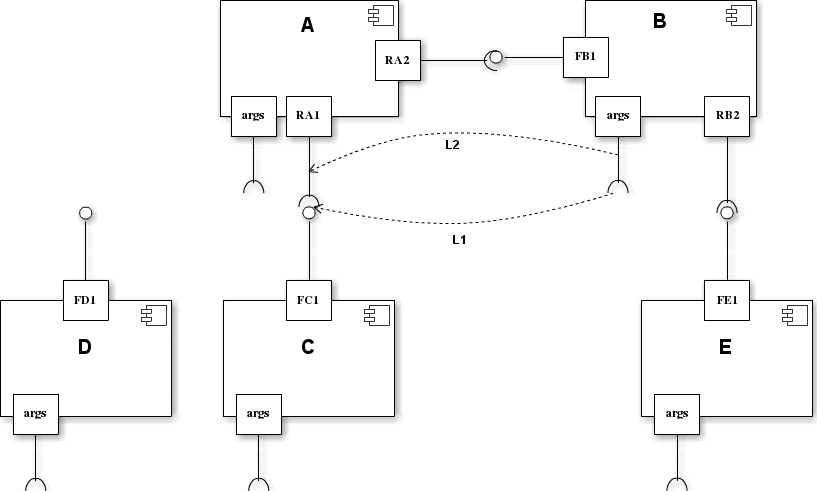
\includegraphics{images/archiCompo.png}
}
\caption{Exemple du passage en arguments d'un composant}
\label{fig:archiCompo}
\end{figure}
  
  \subsection{Les premières pistes du passage d'arguments}
  
      \subsubsection{Le passage par fourni}
      
      Une connexion par port fourni (ou passage par fourni), figure \ref{fig:archiCompo}, représenté par la liaison \emph{L1} entre le port \emph{args[1]} du composant B et le port fournis \emph{FC1} du composant C. Cette connexion entre B et C permet au composant B d'avoir accès au service de C, cependant on remarque que le composant A n'a plus de contrôle sur cette connexion car elle ne passe plus par lui. De plus si jamais le composant A décide de modifier sa connexion à C vers un autre composant (ici D par exemple), alors B gardera la connexion vers C, créant ainsi un comportement parallèle. Ce comportement peut s'avérer utilise dans certain cas, par exemple si A modifie sa connexion plusieurs fois, il permettrait à B de conserver des connexions vers les anciens arguments de A, permettant d'avoir un historique des connexions. 
      
      \subsubsection{Le passage par requis}
      
      Une connexion par port requis (ou passage par requis), figure \ref{fig:archiCompo}, représenté par la liaison \emph{L2} entre le port \emph{args[1]} du composant B et le port requis \emph{RA1} du composant A. Cette liaison met en place un mécanisme de délégation entre le port de A et le port de B. Cela permet à B d'invoquer les services de C, tout en permettant à A d'avoir un possible contrôle sur cette connexion, car elle passe par son port. De plus si jamais A modifie sa connexion à C vers un nouveau composant, alors B aura lui aussi cette connexion vers D. Cela permet donc la création d'architecture très réactive aux changements de composants, ce qui fait défaut au passage par fourni. 
      
  \subsection{Comparaison avec les passages d'arguments classique}
  
  Nous avons vue précédemment les différents mécanismes de passage d'argument qui pouvaient exister dans les langages de programmation. Il est intéressant de se demander comment ces différents mécanismes pourraient se traduire dans un passage de composant en arguments. 
   
  On peut faire un premier parallèle du passage par fourni, qui semble permettre un mécanisme similaire au passage de référence de Java. En effet les modifications de l'état du composant C dans le service de B auront un impact sur le composant C. De plus si A modifie sa connexion vers C vers un autre composant et que B a conservé sa connexion vers C alors comme en Java B n'aura pas une référence vers D mais toujours vers C.
  
  Le passage par requis ne peut pas se réaliser en Java, mais on peut avoir un comportement qui s'en rapproche en C++ par un référencement vers un pointeur. Si une objet A passe par référence un pointeur $c$ à une méthode $foo$ de B, et que B conserve cette référence dans un pointeur $var$, alors $var$ aura comme référence l'adresse du pointeur $c$. Ainsi si A modifie la référence du pointeur $c$, alors B aura bien une référence vers un pointeur qui fera référence à ce nouvelle objet.
  
  \subsection{Les potentialités découlant du passage par requis comme support au passage d'arguments}

    Le passage par requis permet déjà des potentialités sur cette connexion pour le passage en arguments, et qui demanderait peut de modification afin d'être implémenté, déjà simulable manuellement par le programmeur.  
  
      \subsubsection{Un passage en lecture seule}
    
   Une connexion en mode <<read-only>> permettrait en effet de pouvoir passer un composant C à un composant B, où B ne pourrait pas modifier l'état du composant C, c'est-à-dire invoquer seulement des services de C qui non pas un impact sur l'état de C, comparable à l'utilisation du mot clé const de C++. On peut donc imaginer la mise en place d'une nouvelle propriété sur les ports qui indiquerait si ils sont en mode <<read-only>> ou non et de pouvoir modifier cette propriété selon le besoin. On peut aussi imaginer un nouveau type de port qui ne permettrait que le passage en <<read-only>> et le composant A devrait choisir quel type de port il veut utiliser. Ce mécanisme <<read-only>> peut cependant être réalisé manuellement par la mise en place d'un composant placé entre nos deux composants, qui filtrerai les services que peut invoquer notre composant.
  
      \subsubsection{Un passage révocable}
    
    Nous avons vu que le passage par requis permettait au composant A d'exercer un contrôle sur la connexion de B vers C. On peut donc imaginer là aussi une nouvelle propriété ou un nouveau type de port permettant de <<couper>> la connexion entre B et C mais aussi de pouvoir la rétablir selon le besoin. La difficulté de la propagation d'un passage révocable par le passage par requis est minime, si B passe en argument C au composant E, alors supprimer la délégation entre le port de A et le port B, supprimera la délégation implicite de E vers C. \\\par
    
  \subsection{De nouvelles pistes ouvertes par les résultats de récentes recherches}
  
    \subsubsection{Les références comme entité de première classe}
    
    Faire des références une entité de première classe permet d'exercer un contrôle sur les références des objets, permettant de construire des système objets avec une plus grande sécurité. En apportant des comportements comme des références en lecture seule, révocable. On pourra notamment regarder les travaux portant sur les langages à typage statique \cite{clarke1998ownership} ou encore les travaux de \cite{arnaudhandles} portant sur les langages à typage dynamique. 
    
    Cependant on pourra discuter de la propagation du contrôle des références, en regardant un exemple inspiré de \cite{arnaudhandles}. Un objet A passe une référence révocable vers un objet C à un objet B, cependant B a aussi une autre référence indirecte vers C en passant par D. Alors si A révoque la référence révocable vers C, cela a t'il un impact sur la référence indirecte vers B ?
    
    On pourra aussi regrouper les travaux de \cite{abi2006javad}, qui essaye de lutter contre l'aliasing, en contrôlant les échanges de références, en regroupant les objets dans des domaines et en explicitant les lien entre eux. Mettant aussi en place des mots clés, comme \textbf{unique} (ne peut être pointé que par une seule référence), \textbf{owned} (ne peut être accessible que par des objets du même domaine), \textbf{shared} (partagé entre les domaines), permettant de gérer les droits d'accès des objets.
    
    On remarque cependant que ces différents mécanismes se retrouve conceptuellement dans les ports de Compo, et pourrait si implémenté sans demander un grand effort de conception, par l'ajout de nouveaux types de ports par exemple.
    
    \subsubsection{La réification des connecteurs}
       
    Un connecteur permet de représenter la sémantique d'une connexion entre deux ou plusieurs instances. Cependant les langages orientés objets ne permettent pas de fournir une représentation explicite des connections entre instances, car étant implicitement comprit dans leur références. Dans le monde composant cette connexions est explicitement décrite et représent une liaison entre deux ou plusieurs élément connectable (e.g. ports ou interfaces) \cite{IversDocumentingComponent2004}.
    
    \cite{aldrich2003language} propose donc d'intégrer les connecteurs au LOC ArchJava, afin de permettre au développer de pouvoir modifier la sémantique d'un connecteur à l’exécution et de modifier le comportement de vérification de type entre les ports. 
    Par défaut la compatibilité de deux interfaces est la même que dans Java, cependant ajouter un nouveaux connecteur qui hérite de la classe $Connector$ et surcharger sa méthode $typecheck$, permet de modifier la vérification de cette compatibilité. 
    Par exemple, dans \cite{aldrich2003language}, un nouveaux connecteur $TCPConnector$ est définie, ne supportant une conne\-xion qu'entre exactement deux ports et l'ensemble des arguments doivent être des sous-types de l'interfaces $Serialisable$ de Java. Le développeur peut ensuite s'il le désire lors de la définition d'une connections (\textbf{connect}), spécifier un connecteur particulier (\textbf{with new} [{\itshape connecteur}])
    
    Réifier les connecteurs dans Compo ne serait que redondant car leur mécanisme étant déjà incorporé dans les ports. Cependant la possibilité de pouvoir ajouter un nouveaux comportement de vérification peut être utile dans certain besoin d'utilisation et ce réaliserai par l'utilisation d'un nouveau type de port. 

  \subsection{La signification du retour d'un composant à une invocation de service}
  
      En complémentaire des interrogations sur le passage de composants en arguments, il est intéressant se demander se que signifie retourner un composant suite à une invocation de service. Une connexion est aussi réalisé entre le composant retourné et le composant qui réalise l'invocation. On prendra comme exemple, le composant E qui serait le retour d'un invocation de service du composant B par le composant A, figure \ref{fig:archiCompo}.
  
      Dans le cas d'un retour par port fourni (ou retour par fourni), le même mécanisme de connexion est utilisé entre les ports de nos composants. Alors, une connexion entre un port requis de A et le port fournis $FE1$ de E est mise en place, donnant ainsi une connexion directe vers le composant E au composant A sans avoir à passer par B. 
  
      Dans le cas d'un retour par port requis (ou retour par requis), le même mécanisme de délégation est utilisé entre les deux ports requis. Ainsi, une délégation entre un port requis de A et le port requis $RB2$ est mise en place, donnant ainsi à B le contrôle sur la connexion entre A et E.
    
         
